\documentclass[cn,10pt,math=newtx,citestyle=gb7714-2015,bibstyle=gb7714-2015]{elegantbook}

\usepackage{polynom}
\usepackage{float}

\title{历年 CSP 题目解析}
\subtitle{仅为参考练习所用}

\author{lonlyn}
\institute{Shanxi University Algorithm Group}
\date{December 30, 2021}
\version{1.0}

\setcounter{tocdepth}{3}

\cover{cover.jpg}

% 本文档命令
\usepackage{array}
\newcommand{\ccr}[1]{\makecell{{\color{#1}\rule{1cm}{1cm}}}}

\definecolor{customcolor}{RGB}{32,178,170}
\colorlet{coverlinecolor}{customcolor}

\begin{document}

\maketitle
\frontmatter

\chapter*{特别声明}

\markboth{Introduction}{前言}

该书仅供内部学习使用,如果有侵权请联系作者。

信息学竞赛的发展,吸引越来越多的人加入了“卷”的行列。CCF CSP的历年题解在网上也是随处可见,但题解质量参差不齐。很多题解只有标准答案,缺少题目分析;更有甚者无法通过答案,充满了分号大小写问题等错误。

本书的目的是为了实现以下几点:

\begin{itemize}
  \item 提供规范的代码程序。这里的规范,既要具有程序的可读性,也要具备考场的简易性。
  \item 提供多样的解题思路。有些时候,网上的大佬往往一语道破问题求解的思路,但怎么想到的却往往不提。这里力求从部分分开始,逐渐深入,汇集众人智慧,逐步解决难题。
  \item 提供筛选的额外补充。做一道题的目的不是只做一道题,而是可以做到举一反三,但我们常常忽略这一点。
\end{itemize}

感谢 \href{https://github.com/ElegantLaTeX/ElegantBook}{Elegant\LaTeX{}} 提供如此精美的模板,希望这本书能够给大家带来帮助。

\vskip 1.5cm

\begin{flushright}
lonlyn\\
December 30, 2021
\end{flushright}

\tableofcontents

\mainmatter

\chapter{CCF CSP认证总览}

待补充。

% \chapter{第1次认证(2014年03月)}

% \section{题目及设计知识点}

% \section{201403-1}

\subsection*{题目背景}

\subsection*{题目描述}

\subsection*{输入格式}

\subsection*{输出格式}

\subsection*{样例}

\subsection*{子任务}

\subsection*{提示}



% \section{201403-2}

\subsection*{题目背景}

\subsection*{题目描述}

\subsection*{输入格式}

\subsection*{输出格式}

\subsection*{样例}

\subsection*{子任务}

\subsection*{提示}



% \section{201403-3}

\subsection*{题目背景}

\subsection*{题目描述}

\subsection*{输入格式}

\subsection*{输出格式}

\subsection*{样例}

\subsection*{子任务}

\subsection*{提示}



% \section{201403-4}

\subsection*{题目背景}

\subsection*{题目描述}

\subsection*{输入格式}

\subsection*{输出格式}

\subsection*{样例}

\subsection*{子任务}

\subsection*{提示}



% \section{201403-5}

\subsection*{题目背景}

\subsection*{题目描述}

\subsection*{输入格式}

\subsection*{输出格式}

\subsection*{样例}

\subsection*{子任务}

\subsection*{提示}



% \chapter{第2次认证(2014年09月)}

% \section{题目及设计知识点}

% \section{201409-1}

\subsection*{题目背景}

\subsection*{题目描述}

\subsection*{输入格式}

\subsection*{输出格式}

\subsection*{样例}

\subsection*{子任务}

\subsection*{提示}



% \section{201409-2}

\subsection*{题目背景}

\subsection*{题目描述}

\subsection*{输入格式}

\subsection*{输出格式}

\subsection*{样例}

\subsection*{子任务}

\subsection*{提示}



% \section{201409-3}

\subsection*{题目背景}

\subsection*{题目描述}

\subsection*{输入格式}

\subsection*{输出格式}

\subsection*{样例}

\subsection*{子任务}

\subsection*{提示}



% \section{201409-4}

\subsection*{题目背景}

\subsection*{题目描述}

\subsection*{输入格式}

\subsection*{输出格式}

\subsection*{样例}

\subsection*{子任务}

\subsection*{提示}



% \section{201409-5}

\subsection*{题目背景}

\subsection*{题目描述}

\subsection*{输入格式}

\subsection*{输出格式}

\subsection*{样例}

\subsection*{子任务}

\subsection*{提示}

 

% \chapter{第3次认证(2014年12月)}

% \section{题目及设计知识点}

% \section{201412-1}

\subsection*{题目背景}

\subsection*{题目描述}

\subsection*{输入格式}

\subsection*{输出格式}

\subsection*{样例}

\subsection*{子任务}

\subsection*{提示}



% \section{201412-2}

\subsection*{题目背景}

\subsection*{题目描述}

\subsection*{输入格式}

\subsection*{输出格式}

\subsection*{样例}

\subsection*{子任务}

\subsection*{提示}



% \section{201412-3}

\subsection*{题目背景}

\subsection*{题目描述}

\subsection*{输入格式}

\subsection*{输出格式}

\subsection*{样例}

\subsection*{子任务}

\subsection*{提示}



% \section{201412-4}

\subsection*{题目背景}

\subsection*{题目描述}

\subsection*{输入格式}

\subsection*{输出格式}

\subsection*{样例}

\subsection*{子任务}

\subsection*{提示}



% \section{201412-5}

\subsection*{题目背景}

\subsection*{题目描述}

\subsection*{输入格式}

\subsection*{输出格式}

\subsection*{样例}

\subsection*{子任务}

\subsection*{提示}



% \chapter{第4次认证(2015年03月)}

% \section{题目及设计知识点}

% \section{201503-1}

\subsection*{题目背景}

\subsection*{题目描述}

\subsection*{输入格式}

\subsection*{输出格式}

\subsection*{样例}

\subsection*{子任务}

\subsection*{提示}



% \section{201503-2}

\subsection*{题目背景}

\subsection*{题目描述}

\subsection*{输入格式}

\subsection*{输出格式}

\subsection*{样例}

\subsection*{子任务}

\subsection*{提示}



% \section{201503-3}

\subsection*{题目背景}

\subsection*{题目描述}

\subsection*{输入格式}

\subsection*{输出格式}

\subsection*{样例}

\subsection*{子任务}

\subsection*{提示}



% \section{201503-4}

\subsection*{题目背景}

\subsection*{题目描述}

\subsection*{输入格式}

\subsection*{输出格式}

\subsection*{样例}

\subsection*{子任务}

\subsection*{提示}



% \section{201503-5}

\subsection*{题目背景}

\subsection*{题目描述}

\subsection*{输入格式}

\subsection*{输出格式}

\subsection*{样例}

\subsection*{子任务}

\subsection*{提示}



% \chapter{第5次认证(2015年09月)}

% \section{题目及设计知识点}

% \section{201509-1}

\subsection*{题目背景}

\subsection*{题目描述}

\subsection*{输入格式}

\subsection*{输出格式}

\subsection*{样例}

\subsection*{子任务}

\subsection*{提示}



% \section{201509-2}

\subsection*{题目背景}

\subsection*{题目描述}

\subsection*{输入格式}

\subsection*{输出格式}

\subsection*{样例}

\subsection*{子任务}

\subsection*{提示}



% \section{201509-3}

\subsection*{题目背景}

\subsection*{题目描述}

\subsection*{输入格式}

\subsection*{输出格式}

\subsection*{样例}

\subsection*{子任务}

\subsection*{提示}



% \section{201509-4}

\subsection*{题目背景}

\subsection*{题目描述}

\subsection*{输入格式}

\subsection*{输出格式}

\subsection*{样例}

\subsection*{子任务}

\subsection*{提示}



% \section{201509-5}

\subsection*{题目背景}

\subsection*{题目描述}

\subsection*{输入格式}

\subsection*{输出格式}

\subsection*{样例}

\subsection*{子任务}

\subsection*{提示}



% \chapter{第6次认证(2015年12月)}

% \section{题目及设计知识点}

% \section{201512-1}

\subsection*{题目背景}

\subsection*{题目描述}

\subsection*{输入格式}

\subsection*{输出格式}

\subsection*{样例}

\subsection*{子任务}

\subsection*{提示}

 

% \section{201512-2}

\subsection*{题目背景}

\subsection*{题目描述}

\subsection*{输入格式}

\subsection*{输出格式}

\subsection*{样例}

\subsection*{子任务}

\subsection*{提示}



% \section{201512-3}

\subsection*{题目背景}

\subsection*{题目描述}

\subsection*{输入格式}

\subsection*{输出格式}

\subsection*{样例}

\subsection*{子任务}

\subsection*{提示}



% \section{201512-4}

\subsection*{题目背景}

\subsection*{题目描述}

\subsection*{输入格式}

\subsection*{输出格式}

\subsection*{样例}

\subsection*{子任务}

\subsection*{提示}



% \section{201512-5}

\subsection*{题目背景}

\subsection*{题目描述}

\subsection*{输入格式}

\subsection*{输出格式}

\subsection*{样例}

\subsection*{子任务}

\subsection*{提示}



% \chapter{第7次认证(2016年04月)}

% \section{题目及设计知识点}

% \section{201604-1}

\subsection*{题目背景}

\subsection*{题目描述}

\subsection*{输入格式}

\subsection*{输出格式}

\subsection*{样例}

\subsection*{子任务}

\subsection*{提示}



% \section{201604-2}

\subsection*{题目背景}

\subsection*{题目描述}

\subsection*{输入格式}

\subsection*{输出格式}

\subsection*{样例}

\subsection*{子任务}

\subsection*{提示}



% \section{201604-3}

\subsection*{题目背景}

\subsection*{题目描述}

\subsection*{输入格式}

\subsection*{输出格式}

\subsection*{样例}

\subsection*{子任务}

\subsection*{提示}



% \section{201604-4}

\subsection*{题目背景}

\subsection*{题目描述}

\subsection*{输入格式}

\subsection*{输出格式}

\subsection*{样例}

\subsection*{子任务}

\subsection*{提示}



% \section{201604-5}

\subsection*{题目背景}

\subsection*{题目描述}

\subsection*{输入格式}

\subsection*{输出格式}

\subsection*{样例}

\subsection*{子任务}

\subsection*{提示}



% \chapter{第8次认证(2016年09月)}

% \section{题目及设计知识点}

% \section{201609-1}

\subsection*{题目背景}

\subsection*{题目描述}

\subsection*{输入格式}

\subsection*{输出格式}

\subsection*{样例}

\subsection*{子任务}

\subsection*{提示}



% \section{201609-2}

\subsection*{题目背景}

\subsection*{题目描述}

\subsection*{输入格式}

\subsection*{输出格式}

\subsection*{样例}

\subsection*{子任务}

\subsection*{提示}



% \section{201609-3}

\subsection*{题目背景}

\subsection*{题目描述}

\subsection*{输入格式}

\subsection*{输出格式}

\subsection*{样例}

\subsection*{子任务}

\subsection*{提示}



% \section{201609-4}

\subsection*{题目背景}

\subsection*{题目描述}

\subsection*{输入格式}

\subsection*{输出格式}

\subsection*{样例}

\subsection*{子任务}

\subsection*{提示}



% \section{201609-5}

\subsection*{题目背景}

\subsection*{题目描述}

\subsection*{输入格式}

\subsection*{输出格式}

\subsection*{样例}

\subsection*{子任务}

\subsection*{提示}



% \chapter{第9次认证(2016年12月)}

% \section{题目及设计知识点}

% \section{201612-1}

\subsection*{题目背景}

\subsection*{题目描述}

\subsection*{输入格式}

\subsection*{输出格式}

\subsection*{样例}

\subsection*{子任务}

\subsection*{提示}



% \section{201612-2}

\subsection*{题目背景}

\subsection*{题目描述}

\subsection*{输入格式}

\subsection*{输出格式}

\subsection*{样例}

\subsection*{子任务}

\subsection*{提示}



% \section{201612-3}

\subsection*{题目背景}

\subsection*{题目描述}

\subsection*{输入格式}

\subsection*{输出格式}

\subsection*{样例}

\subsection*{子任务}

\subsection*{提示}



% \section{201612-4}

\subsection*{题目背景}

\subsection*{题目描述}

\subsection*{输入格式}

\subsection*{输出格式}

\subsection*{样例}

\subsection*{子任务}

\subsection*{提示}



% \section{201612-5}

\subsection*{题目背景}

\subsection*{题目描述}

\subsection*{输入格式}

\subsection*{输出格式}

\subsection*{样例}

\subsection*{子任务}

\subsection*{提示}



% \chapter{第10次认证(2017年03月)}

% \section{题目及设计知识点}

% \section{201703-1}

\subsection*{题目背景}

\subsection*{题目描述}

\subsection*{输入格式}

\subsection*{输出格式}

\subsection*{样例}

\subsection*{子任务}

\subsection*{提示}



% \section{201703-2}

\subsection*{题目背景}

\subsection*{题目描述}

\subsection*{输入格式}

\subsection*{输出格式}

\subsection*{样例}

\subsection*{子任务}

\subsection*{提示}



% \section{201703-3}

\subsection*{题目背景}

\subsection*{题目描述}

\subsection*{输入格式}

\subsection*{输出格式}

\subsection*{样例}

\subsection*{子任务}

\subsection*{提示}



% \section{201703-4}

\subsection*{题目背景}

\subsection*{题目描述}

\subsection*{输入格式}

\subsection*{输出格式}

\subsection*{样例}

\subsection*{子任务}

\subsection*{提示}



% \section{201703-5}

\subsection*{题目背景}

\subsection*{题目描述}

\subsection*{输入格式}

\subsection*{输出格式}

\subsection*{样例}

\subsection*{子任务}

\subsection*{提示}



% \chapter{第11次认证(2017年09月)}

% \section{题目及设计知识点}

% \section{201709-1}

\subsection*{题目背景}

\subsection*{题目描述}

\subsection*{输入格式}

\subsection*{输出格式}

\subsection*{样例}

\subsection*{子任务}

\subsection*{提示}



% \section{201709-2}

\subsection*{题目背景}

\subsection*{题目描述}

\subsection*{输入格式}

\subsection*{输出格式}

\subsection*{样例}

\subsection*{子任务}

\subsection*{提示}



% \section{201709-3}

\subsection*{题目背景}

\subsection*{题目描述}

\subsection*{输入格式}

\subsection*{输出格式}

\subsection*{样例}

\subsection*{子任务}

\subsection*{提示}



% \section{201709-4}

\subsection*{题目背景}

\subsection*{题目描述}

\subsection*{输入格式}

\subsection*{输出格式}

\subsection*{样例}

\subsection*{子任务}

\subsection*{提示}



% \section{201709-5}

\subsection*{题目背景}

\subsection*{题目描述}

\subsection*{输入格式}

\subsection*{输出格式}

\subsection*{样例}

\subsection*{子任务}

\subsection*{提示}



% \chapter{第12次认证(2017年12月)}

% \section{题目及设计知识点}

% \section{201712-1}

\subsection*{题目背景}

\subsection*{题目描述}

\subsection*{输入格式}

\subsection*{输出格式}

\subsection*{样例}

\subsection*{子任务}

\subsection*{提示}



% \section{201712-2}

\subsection*{题目背景}

\subsection*{题目描述}

\subsection*{输入格式}

\subsection*{输出格式}

\subsection*{样例}

\subsection*{子任务}

\subsection*{提示}



% \section{201712-3}

\subsection*{题目背景}

\subsection*{题目描述}

\subsection*{输入格式}

\subsection*{输出格式}

\subsection*{样例}

\subsection*{子任务}

\subsection*{提示}



% \section{201712-4}

\subsection*{题目背景}

\subsection*{题目描述}

\subsection*{输入格式}

\subsection*{输出格式}

\subsection*{样例}

\subsection*{子任务}

\subsection*{提示}



% \section{201712-5}

\subsection*{题目背景}

\subsection*{题目描述}

\subsection*{输入格式}

\subsection*{输出格式}

\subsection*{样例}

\subsection*{子任务}

\subsection*{提示}



% \chapter{第13次认证(2018年03月)}

% \section{题目及设计知识点}

% \section{201803-1}

\subsection*{题目背景}

\subsection*{题目描述}

\subsection*{输入格式}

\subsection*{输出格式}

\subsection*{样例}

\subsection*{子任务}

\subsection*{提示}



% \section{201803-2}

\subsection*{题目背景}

\subsection*{题目描述}

\subsection*{输入格式}

\subsection*{输出格式}

\subsection*{样例}

\subsection*{子任务}

\subsection*{提示}



% \section{201803-3}

\subsection*{题目背景}

\subsection*{题目描述}

\subsection*{输入格式}

\subsection*{输出格式}

\subsection*{样例}

\subsection*{子任务}

\subsection*{提示}



% \section{201803-4}

\subsection*{题目背景}

\subsection*{题目描述}

\subsection*{输入格式}

\subsection*{输出格式}

\subsection*{样例}

\subsection*{子任务}

\subsection*{提示}



% \section{201803-5}

\subsection*{题目背景}

\subsection*{题目描述}

\subsection*{输入格式}

\subsection*{输出格式}

\subsection*{样例}

\subsection*{子任务}

\subsection*{提示}



% \chapter{第14次认证(2018年09月)}

% \section{题目及设计知识点}

% \section{201809-1}

\subsection*{题目背景}

\subsection*{题目描述}

\subsection*{输入格式}

\subsection*{输出格式}

\subsection*{样例}

\subsection*{子任务}

\subsection*{提示}



% \section{201809-2}

\subsection*{题目背景}

\subsection*{题目描述}

\subsection*{输入格式}

\subsection*{输出格式}

\subsection*{样例}

\subsection*{子任务}

\subsection*{提示}



% \section{201809-3}

\subsection*{题目背景}

\subsection*{题目描述}

\subsection*{输入格式}

\subsection*{输出格式}

\subsection*{样例}

\subsection*{子任务}

\subsection*{提示}



% \section{201809-4}

\subsection*{题目背景}

\subsection*{题目描述}

\subsection*{输入格式}

\subsection*{输出格式}

\subsection*{样例}

\subsection*{子任务}

\subsection*{提示}



% \section{201809-5}

\subsection*{题目背景}

\subsection*{题目描述}

\subsection*{输入格式}

\subsection*{输出格式}

\subsection*{样例}

\subsection*{子任务}

\subsection*{提示}



% \chapter{第15次认证(2018年12月)}

% \section{题目及设计知识点}

% \section{201812-1}

\subsection*{题目背景}

\subsection*{题目描述}

\subsection*{输入格式}

\subsection*{输出格式}

\subsection*{样例}

\subsection*{子任务}

\subsection*{提示}



% \section{201812-2}

\subsection*{题目背景}

\subsection*{题目描述}

\subsection*{输入格式}

\subsection*{输出格式}

\subsection*{样例}

\subsection*{子任务}

\subsection*{提示}



% \section{201812-3}

\subsection*{题目背景}

\subsection*{题目描述}

\subsection*{输入格式}

\subsection*{输出格式}

\subsection*{样例}

\subsection*{子任务}

\subsection*{提示}



% \section{201812-4}

\subsection*{题目背景}

\subsection*{题目描述}

\subsection*{输入格式}

\subsection*{输出格式}

\subsection*{样例}

\subsection*{子任务}

\subsection*{提示}



% \section{201812-5}

\subsection*{题目背景}

\subsection*{题目描述}

\subsection*{输入格式}

\subsection*{输出格式}

\subsection*{样例}

\subsection*{子任务}

\subsection*{提示}



% \chapter{第16次认证(2019年03月)}

% \section{题目及设计知识点}

% \section{201903-1}

\subsection*{题目背景}

\subsection*{题目描述}

\subsection*{输入格式}

\subsection*{输出格式}

\subsection*{样例}

\subsection*{子任务}

\subsection*{提示}



% \section{201903-2}

\subsection*{题目背景}

\subsection*{题目描述}

\subsection*{输入格式}

\subsection*{输出格式}

\subsection*{样例}

\subsection*{子任务}

\subsection*{提示}



% \section{201903-3}

\subsection*{题目背景}

\subsection*{题目描述}

\subsection*{输入格式}

\subsection*{输出格式}

\subsection*{样例}

\subsection*{子任务}

\subsection*{提示}



% \section{201903-4}

\subsection*{题目背景}

\subsection*{题目描述}

\subsection*{输入格式}

\subsection*{输出格式}

\subsection*{样例}

\subsection*{子任务}

\subsection*{提示}



% \section{201903-5}

\subsection*{题目背景}

\subsection*{题目描述}

\subsection*{输入格式}

\subsection*{输出格式}

\subsection*{样例}

\subsection*{子任务}

\subsection*{提示}



% \chapter{第17次认证(2019年09月)}

% \section{题目及设计知识点}

% \section{201909-1}

\subsection*{题目背景}

\subsection*{题目描述}

\subsection*{输入格式}

\subsection*{输出格式}

\subsection*{样例}

\subsection*{子任务}

\subsection*{提示}



% \section{201909-2}

\subsection*{题目背景}

\subsection*{题目描述}

\subsection*{输入格式}

\subsection*{输出格式}

\subsection*{样例}

\subsection*{子任务}

\subsection*{提示}



% \section{201909-3}

\subsection*{题目背景}

\subsection*{题目描述}

\subsection*{输入格式}

\subsection*{输出格式}

\subsection*{样例}

\subsection*{子任务}

\subsection*{提示}



% \section{201909-4}

\subsection*{题目背景}

\subsection*{题目描述}

\subsection*{输入格式}

\subsection*{输出格式}

\subsection*{样例}

\subsection*{子任务}

\subsection*{提示}



% \section{201909-5}

\subsection*{题目背景}

\subsection*{题目描述}

\subsection*{输入格式}

\subsection*{输出格式}

\subsection*{样例}

\subsection*{子任务}

\subsection*{提示}



% \chapter{第18次认证(2019年12月)}

% \section{题目及设计知识点}

% \section{201912-1}

\subsection*{题目背景}

\subsection*{题目描述}

\subsection*{输入格式}

\subsection*{输出格式}

\subsection*{样例}

\subsection*{子任务}

\subsection*{提示}



% \section{201912-2}

\subsection*{题目背景}

\subsection*{题目描述}

\subsection*{输入格式}

\subsection*{输出格式}

\subsection*{样例}

\subsection*{子任务}

\subsection*{提示}



% \section{201912-3}

\subsection*{题目背景}

\subsection*{题目描述}

\subsection*{输入格式}

\subsection*{输出格式}

\subsection*{样例}

\subsection*{子任务}

\subsection*{提示}



% \section{201912-4}

\subsection*{题目背景}

\subsection*{题目描述}

\subsection*{输入格式}

\subsection*{输出格式}

\subsection*{样例}

\subsection*{子任务}

\subsection*{提示}



% \section{201912-5}

\subsection*{题目背景}

\subsection*{题目描述}

\subsection*{输入格式}

\subsection*{输出格式}

\subsection*{样例}

\subsection*{子任务}

\subsection*{提示}



% \chapter{第19次认证(2020年06月)}

% \section{题目及设计知识点}

% \section{202006-1}

\subsection*{题目背景}

\subsection*{题目描述}

\subsection*{输入格式}

\subsection*{输出格式}

\subsection*{样例}

\subsection*{子任务}

\subsection*{提示}



% \section{202006-2}

\subsection*{题目背景}

\subsection*{题目描述}

\subsection*{输入格式}

\subsection*{输出格式}

\subsection*{样例}

\subsection*{子任务}

\subsection*{提示}



% \section{202006-3}

\subsection*{题目背景}

\subsection*{题目描述}

\subsection*{输入格式}

\subsection*{输出格式}

\subsection*{样例}

\subsection*{子任务}

\subsection*{提示}



% \section{202006-4}

\subsection*{题目背景}

\subsection*{题目描述}

\subsection*{输入格式}

\subsection*{输出格式}

\subsection*{样例}

\subsection*{子任务}

\subsection*{提示}



% \section{202006-5}

\subsection*{题目背景}

\subsection*{题目描述}

\subsection*{输入格式}

\subsection*{输出格式}

\subsection*{样例}

\subsection*{子任务}

\subsection*{提示}



% \chapter{第20次认证(2020年09月)}

% \section{题目及设计知识点}

% \section{202009-1}

\subsection*{题目背景}

\subsection*{题目描述}

\subsection*{输入格式}

\subsection*{输出格式}

\subsection*{样例}

\subsection*{子任务}

\subsection*{提示}



% \section{202009-2}

\subsection*{题目背景}

\subsection*{题目描述}

\subsection*{输入格式}

\subsection*{输出格式}

\subsection*{样例}

\subsection*{子任务}

\subsection*{提示}



% \section{202009-3}

\subsection*{题目背景}

\subsection*{题目描述}

\subsection*{输入格式}

\subsection*{输出格式}

\subsection*{样例}

\subsection*{子任务}

\subsection*{提示}



% \section{202009-4}

\subsection*{题目背景}

\subsection*{题目描述}

\subsection*{输入格式}

\subsection*{输出格式}

\subsection*{样例}

\subsection*{子任务}

\subsection*{提示}



% \section{202009-5}

\subsection*{题目背景}

\subsection*{题目描述}

\subsection*{输入格式}

\subsection*{输出格式}

\subsection*{样例}

\subsection*{子任务}

\subsection*{提示}



% \chapter{第21次认证(2020年12月)}

% \section{题目及设计知识点}

% \section{202012-1}

\subsection*{题目背景}

\subsection*{题目描述}

\subsection*{输入格式}

\subsection*{输出格式}

\subsection*{样例}

\subsection*{子任务}

\subsection*{提示}



% \section{202012-2}

\subsection*{题目背景}

\subsection*{题目描述}

\subsection*{输入格式}

\subsection*{输出格式}

\subsection*{样例}

\subsection*{子任务}

\subsection*{提示}



% \section{202012-3}

\subsection*{题目背景}

\subsection*{题目描述}

\subsection*{输入格式}

\subsection*{输出格式}

\subsection*{样例}

\subsection*{子任务}

\subsection*{提示}



% \section{202012-4}

\subsection*{题目背景}

\subsection*{题目描述}

\subsection*{输入格式}

\subsection*{输出格式}

\subsection*{样例}

\subsection*{子任务}

\subsection*{提示}



% \section{202012-5}

\subsection*{题目背景}

\subsection*{题目描述}

\subsection*{输入格式}

\subsection*{输出格式}

\subsection*{样例}

\subsection*{子任务}

\subsection*{提示}



% \chapter{第22次认证(2021年04月)}

% \section{题目及设计知识点}

% \section{202104-1}

\subsection*{题目背景}

\subsection*{题目描述}

\subsection*{输入格式}

\subsection*{输出格式}

\subsection*{样例}

\subsection*{子任务}

\subsection*{提示}



% \section{202104-2}

\subsection*{题目背景}

\subsection*{题目描述}

\subsection*{输入格式}

\subsection*{输出格式}

\subsection*{样例}

\subsection*{子任务}

\subsection*{提示}



% \section{202104-3}

\subsection*{题目背景}

\subsection*{题目描述}

\subsection*{输入格式}

\subsection*{输出格式}

\subsection*{样例}

\subsection*{子任务}

\subsection*{提示}



% \section{202104-4}

\subsection*{题目背景}

\subsection*{题目描述}

\subsection*{输入格式}

\subsection*{输出格式}

\subsection*{样例}

\subsection*{子任务}

\subsection*{提示}



% \section{202104-5}

\subsection*{题目背景}

\subsection*{题目描述}

\subsection*{输入格式}

\subsection*{输出格式}

\subsection*{样例}

\subsection*{子任务}

\subsection*{提示}



% \chapter{第23次认证(2021年09月)}

% \section{题目及设计知识点}

% \section{202109-1}

\subsection*{题目背景}

\subsection*{题目描述}

\subsection*{输入格式}

\subsection*{输出格式}

\subsection*{样例}

\subsection*{子任务}

\subsection*{提示}



% \section{202109-2}

\subsection*{题目背景}

\subsection*{题目描述}

\subsection*{输入格式}

\subsection*{输出格式}

\subsection*{样例}

\subsection*{子任务}

\subsection*{提示}



% \section{202109-3}

\subsection*{题目背景}

\subsection*{题目描述}

\subsection*{输入格式}

\subsection*{输出格式}

\subsection*{样例}

\subsection*{子任务}

\subsection*{提示}



% \section{202109-4}

\subsection*{题目背景}

\subsection*{题目描述}

\subsection*{输入格式}

\subsection*{输出格式}

\subsection*{样例}

\subsection*{子任务}

\subsection*{提示}



% \section{202109-5}

\subsection*{题目背景}

\subsection*{题目描述}

\subsection*{输入格式}

\subsection*{输出格式}

\subsection*{样例}

\subsection*{子任务}

\subsection*{提示}



\chapter{第24次认证(2021年12月)}

\section{题目及涉及知识点}

\begin{table}[htbp]
  \centering
  \begin{tabular}{ccc}
    \toprule
    题目编号 & 题目名称 & 知识点\\
    \midrule
    1 & 序列查询 & 数学\\
    2 & 序列查询新解 & 数学\\
    3 & 登机牌条码 & 模拟,多项式除法\\
    4 & 磁盘文件操作 & 线段树\\
    5 & 极差路径 & 树分治\\
    \bottomrule
  \end{tabular}
\end{table}

\section{202112-1 序列查询}

\subsection*{题目背景}

西西艾弗岛的购物中心里店铺林立,商品琳琅满目。为了帮助游客根据自己的预算快速选择心仪的商品,IT 部门决定研发一套商品检索系统,支持对任意给定的预算 $x$,查询在该预算范围内($\le x$)价格最高的商品。如果没有商品符合该预算要求,便向游客推荐可以免费领取的西西艾弗岛定制纪念品。

假设购物中心里有 $n$ 件商品,价格从低到高依次为 $A_1,A_2,\cdots, A_n$,
,则根据预算 $x$ 检索商品的过程可以抽象为如下序列查询问题。

\subsection*{题目描述}

$A=[A_0,A_1,A_2,\cdots,A_n]$ 是一个由 $n+1$ 个 $[0,N)$ 范围内整数组成的序列,满足 $0=A_0<A_1<A_2<\cdots<A_n<N$
。(这个定义中蕴含了 $n$ 一定小于 $N$。)

基于序列 $A$,对于 $[0,N)$ 范围内任意的整数 $x$,查询 $f(x)$ 定义为:序列 $A$ 中{\heiti 小于等于} $x$ 的整数里最大的数的{\heiti 下标}。具体来说有以下两种情况:

\begin{enumerate}
  \item 存在下标 $0\le i<n$ 满足 $A_i\le x < A_{i+1}$,此时序列 $A$ 中从 $A_0$ 到 $A_i$ 均小于等于 $x$,其中最大的数为 $A_i$,其下标为 $i$,故 $f(x)=i$。
  \item $A_n\le x$,此时序列 $A$ 中左右的数都小于等于 $x$,其中最大的数是 $A_n$,故 $f(x)=n$。
\end{enumerate}

令 $sum(A)$ 表示 $f(0)$ 到 $f(N-1)$ 的总和,即:

\begin{equation*}
sum(A) = \sum_{i=0}^{N-1} {f(i)=f(0)+f(1)+f(2)+\cdots +f(N-1)}
\end{equation*}

对于给定的序列 $A$,试计算 $sum(A)$。

\subsection*{输入格式}

从标准输入读入数据。

输入的第一行包含空格分隔的两个正整数 $n$ 和 $N$。

输入的第二行包含 $n$ 个用空格分隔的整数 $A_1,A_2,\cdots,A_n$
。

注意 $A_0$
 固定为 $0$,因此输入数据中不包括 $A_0$ 
。

\subsection*{输出格式}

输出到标准输出。

仅输出一个整数,表示 $sum(A)$ 的值。

\subsection*{样例}

输入\#1:

\begin{lstlisting}
3 10
2 5 8
\end{lstlisting}

输出\#1:

\begin{lstlisting}
15
\end{lstlisting}

解释\#1:

$A=[0, 2, 5, 8]$

\begin{table}[H]
  \centering
  \begin{tabular}{ccccccccccc}
    \toprule
    $i$ & $0$ & $1$ & $2$ & $3$ & $4$ & $5$ & $6$ & $7$ & $8$ & $9$ \\
    $f(i)$ & $0$ & $0$ & $1$ & $1$ & $1$ & $2$ & $2$ & $2$ & $3$ & $3$ \\
    \bottomrule
  \end{tabular}
\end{table}

如上表所示,$sum(A)=f(0)+f(1)+\cdots + f(9)=15$。

考虑到 $f(0)=f(1)$、$f(2)=f(3)=f(4)$、$f(5)=f(6)=f(7)$ 以及 $f(8)=f(9)$,亦可通过如下算式计算 $sum(A)$;

\begin{equation*}
  sum(A)=f(0)\times 2+f(2)\times 3+f(5)\times 3 + f(8)\times 2
\end{equation*}

输入\#2:

\begin{lstlisting}
9 10
1 2 3 4 5 6 7 8 9
\end{lstlisting}

输出\#2:

\begin{lstlisting}
45
\end{lstlisting}

\subsection*{子任务}

$50$ \% 的测试数据满足 $1\le n\le 200$ 且 $n\le N\le 1000$;

全部的测试数据满足 $1\le n\le 200$ 且 $n\le N\le 10^7$。

\subsection*{提示}

若存在区间 $[i,j)$ 满足 $f(i)=f(i+1)=\cdots=f(j-1)$,使用乘法运算 $f(i)\times (j-i)$ 代替将 $f(i)$ 到 $f(j-1)$ 逐个相加,或可大幅提高算法效率。


\subsection{$50$\% 数据——模拟}

\subsubsection{思路}

模拟一下这个过程,计算出每一个 $f(i)$ 后加起来即可。

考虑针对确定的 $x$,如何求解 $f(x)$。我们可以从小到大枚举 $A$ 中的数,枚举到第一个大于等于 $x$ 的数即可。注意末尾的判断。

枚举 $x$ 时间复杂度 $\mathbf{O}(N)$,计算 $f(x)$ 时间复杂度 $\mathbf{O}(n)$,整体时间复杂度 $\mathbf{O}(nN)$。

\subsubsection{C++实现}

待补充。

\subsection{$100$\% 数据——利用 $f(x)$ 单调性}

\subsubsection{思路}

为了方便,设 $f(n+1) = \infty$。

通过模拟,可以得到一个显然的结论:

\begin{theorem}[$f(x)$的单调性] \label{thm:fx_monotonicity} 
  对于 $x,y\in [0,N)$,若 $x \le y$,则 $f(x) \le f(y)$。
\end{theorem}

那么,我们可以从小到大枚举 $x$,同时记录目前 $f(x)$ 的值,设为 $y$,那么 $A_{y+1}$ 是第一个大于 $x$ 的数。
当需要计算 $f(x+1)$ 的时候,我们从小到大依次判断 $A_{y+1},A_{y+2},\cdots$ 是否满足条件,
直到遇到第一个大于 $f(x+1)$ 的数 $A_z$,那么 $f(x+1)=z-1$。
之后,在 $f(x+1)$ 的基础上以同样的步骤求 $f(x+2)$,直到求完所有的值。

考虑该算法的时间复杂度,枚举 $x$ 的复杂度是 $\mathbf{O}(N)$,
而 $A$ 数组中每个数对多被枚举一次,枚举所有 $x$ 的整体复杂度 $\mathbf{O}(n)$,
可以得到整体复杂度 $\mathbf{O}(N+n)$。

\subsubsection{C++实现}

\lstinputlisting[language=c++]{code/24/202112-1-100.cpp}

\subsection{$100$\% 数据——阶段求和}

\subsubsection{思路}

在提示中,指出了可以将 $f(x)$ 相同的值一起计算。现在需要解决的问题是如何快速确定 $f(x)$ 值相等的区间。

通过观察和模拟可以发现,随着 $x$ 增大,$f(x)$ 只会在等于某个 $A$ 数组的值时发生变化。
更具体的说,对于某个属于 $A$ 数组的值 $A_i$ 来说,$[A_i,A_{i+1}-1]$ 间的 $f(x)$ 值是相同的,
这样的数共有 $A_{i+1}-A_i$ 个。

也可以以另一种方式理解:对于一个值 $y$,考虑有多少 $x$ 满足 $f(x)=y$。
当 $x<A_y$ 时,$f(x)<y$,当 $x\ge A_{y+1}$ 时,$f(x)>y$。
只有 $x\in [A_y,A_{y+1}]$ 时才能得到 $f(x)=y$。

得到范围后,我们就可以根据 $A$ 数组来进行求和计算。

考虑 $f(x)=n$ 的处理:
我们可以得知满足 $f(x)=n$ 的 $x$ 共有 $N-A_n$ 个,
根据上文推算,我们可以将 $A_{n+1}$ 设置为 $A_n+(N-A_n)=N$ 即可等效替代。

时间复杂度 $\mathbf{O}(n)$。

\subsubsection{C++实现}

\lstinputlisting[language=c++]{code/24/202112-1-100-2.cpp}

\section{202112-2 序列查询新解}

\subsection*{题目背景}

上一题“序列查询”中说道:
$A=[A_0,A_1,A_2,\cdots,A_n]$ 是一个由 $n+1$ 个 $[0,N)$ 范围内整数组成的序列,满足 $0 = A_0 < A_1 < A_2 < \cdots < A_n < N$
。基于序列 $A$,对于 $[0,N)$ 范围内任意的整数 $x$,查询 $f(x)$ 定义为:序列 $A$ 中{\heiti{小于等于}} $x$ 的整数里最大的数的下标。

对于给定的序列 $A$ 和整数 $x$,查询 $f(x)$ 是一个很经典的问题,可以使用二分搜索在 $\mathbf{O}(\log n)$ 的时间复杂度内轻松解决。但在 IT 部门讨论如何实现这一功能时,小 P 同学提出了些新的想法。

\subsection*{题目描述}

小 P 同学认为,如果事先知道了序列 $A$ 中整数的分布情况,就能直接估计出其中小于等于 $x$ 的最大整数的大致位置。接着从这一估计位置开始线性查找,锁定 $f(x)$。如果估计得足够准确,线性查找的时间开销可能比二分查找算法更小。

比如说,如果 $A_1,A_2,\cdots,A_n$
 均匀分布在 $(0,N)$ 的区间,那么就可以估算出:
 
\begin{equation*}
    f(x)\approx \frac{(n+1)\cdot x}{N}
\end{equation*}

为了方便计算,小 P 首先定义了比例系数 $r=\lfloor \frac{N}{n+1} \rfloor$
 
,其中 $\lfloor \rfloor$ 表示下取整,即 $r$ 等于 $N$ 除以 $n+1$ 的商。进一步地,小 P 用 $g(x)=\lfloor \frac{x}{r}\rfloor$
 
 表示自己估算出的 $f(x)$ 的大小,这里同样使用了下取整来保证 $g(x)$ 是一个整数。

显然,对于任意的询问 $x\in [0,N)$,$g(x)$ 和 $f(x)$ 越接近则说明小 P 的估计越准确,后续进行线性查找的时间开销也越小。因此,小 P 用两者差的绝对值 $|g(x)-f(x)|$ 来表示处理询问 $x$ 时的误差。

为了整体评估小 P 同学提出的方法在序列 $A$ 上的表现,试计算:
 
\begin{equation*}
    error(A)=\sum\limits_{i=0}^{N-1}{|g(i)-f(i)|}=|g(0)-f(0)| + \cdots + |g(N-1)-f(N-1)|
\end{equation*}

\subsection*{输入格式}

从标准输入读入数据。

输入的第一行包含空格分隔的两个正整数 $n$ 和 $N$。

输入的第二行包含 $n$ 个用空格分隔的整数 $A_1,A_2,\cdots,A_n$
。

注意 $A_0$
 固定为 $0$,因此输入数据中不包括 $A_0$
。

\subsection*{输出格式}

输出到标准输出。

仅输出一个整数,表示 $error(A)$ 的值。

\subsection*{样例}

输入格式\#1:

\begin{lstlisting}
3 10
2 5 8
\end{lstlisting}

输出格式\#1:

\begin{lstlisting}
5
\end{lstlisting}

解释\#1:

$A=[0, 2, 5, 8]$

$r = \lfloor \frac{N}{n+1}\rfloor=\lfloor \frac{10}{3+1}\rfloor=2$

\begin{table}[H]
  \centering
  \begin{tabular}{ccccccccccc}
    \toprule
    % \midrule
    $i$ & $0$ & $1$ & $2$ & $3$ & $4$ & $5$ & $6$ & $7$ & $8$ & $9$ \\
    $f(i)$ & $0$ & $0$ & $1$ & $1$ & $1$ & $2$ & $2$ & $2$ & $3$ & $3$ \\
    $g(i)$ & $0$ & $0$ & $1$ & $1$ & $2$ & $2$ & $3$ & $3$ & $4$ & $4$ \\
    $|g(i)-f(i)|$ & $0$ & $0$ & $0$ & $0$ & $1$ & $0$ & $1$ & $1$ & $1$ & $1$ \\
    \bottomrule
  \end{tabular}
\end{table}

输入格式\#2:

\begin{lstlisting}
9 10
1 2 3 4 5 6 7 8 9
\end{lstlisting}

输出格式\#2:

\begin{lstlisting}
0
\end{lstlisting}

输入格式\#3:

\begin{lstlisting}
2 10
1 3
\end{lstlisting}

输出格式\#3:

\begin{lstlisting}
6
\end{lstlisting}

解释\#3:

$A=[0, 1, 3]$

$r = \lfloor \frac{N}{n+1}\rfloor=\lfloor \frac{10}{2+1}\rfloor=3$

\begin{table}[H]
  \centering
  \begin{tabular}{ccccccccccc}
    \toprule
    % \midrule
    $i$ & $0$ & $1$ & $2$ & $3$ & $4$ & $5$ & $6$ & $7$ & $8$ & $9$ \\
    $f(i)$ & $0$ & $1$ & $1$ & $2$ & $2$ & $2$ & $2$ & $2$ & $2$ & $2$ \\
    $g(i)$ & $0$ & $0$ & $0$ & $1$ & $1$ & $1$ & $2$ & $2$ & $2$ & $3$ \\
    $|g(i)-f(i)|$ & $0$ & $1$ & $1$ & $1$ & $1$ & $1$ & $0$ & $0$ & $0$ & $1$ \\
    \bottomrule
  \end{tabular}
\end{table}

\subsection*{子任务}

$70$ \% 的测试数据满足 $1\le n\le 200$ 且 $n\le N\le 1000$;

全部的测试数据满足 $1\le n\le 10^5$ 且 $n\le N\le 10^9$。

\subsection*{提示}

需要注意,输入数据 $[A_1\cdots A_n]$
 并不一定均匀分布在 $(0,N)$ 区间,因此总误差 $error(A)$ 可能很大。



\section{202112-3 登机牌条码}

\subsection*{题目背景}

西西艾弗岛景色优美,游人如织。
但是,由于和外界的交通只能靠渡船,交通的不便严重制约了岛上旅游业的发展。
西西艾弗岛管委会经过努力,争取到了一笔投资,建设了一个通用航空机场。
在三年紧锣密鼓的主体建设后,西西艾弗岛通用航空机场终于开始进行航站楼内部软硬件系统的安装和调试工程了。
小 C 是机场运营公司信息部的研发工程师,最近,信息部门的一项重要任务是,研发登机牌自助打印系统。
如图所示的是设计部门根据国际民航组织的行业标准设计的登机牌样张。

\begin{figure}[H]
    \centering
    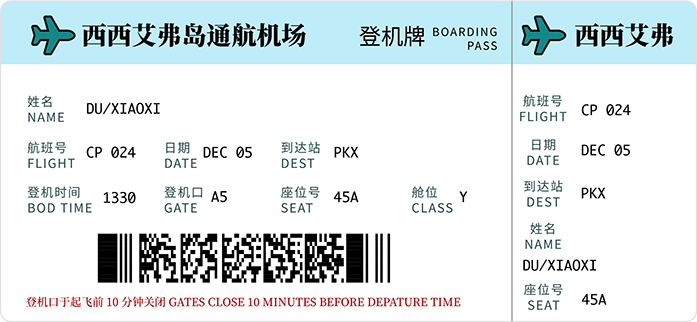
\includegraphics[width=0.95\textwidth]{image/24/3-p-1.png}
\end{figure}

登机牌上最重要的部分就是最下方的机读条形码了。小 C 承担了生成机读条形码算法的开发工作。从被编码的数据到条形码,中间有好多步骤要走。小 C 请你来帮忙,让你帮忙处理一下数据编码的问题。

\subsection*{题目描述}

登机牌上的条形码,是 PDF417 码。PDF417 码的结构如下图所示。

\begin{figure}[H]
    \centering
    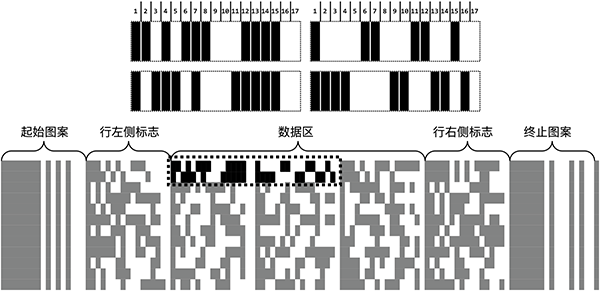
\includegraphics[width=0.95\textwidth]{image/24/3-p-2.png}
\end{figure}

PDF417 码组成的基本元素是码元(Module),所有的码元都是等大的矩形,填充有黑色或白色。码元先组成行,若干行堆叠组成整个 PDF417 码。每一行中,每 17 个码元表示一个{\heiti{码字}}(Code word)。码字是 PDF417 编码中的最小数据单位。每个码字图案中,有交替排列的四个黑色矩形和四个白色矩形,这便是 “417” 的由来。每行开始和结尾有固定的起始和中止图案。与他们相邻的是行左侧和右侧标志,表示行号、行内码字个数等信息。中间的是有效数据区。编码的步骤是:先按照编码规则,将被编码的数据转换为码字;接着根据选定 PDF417 码的宽度(即每行码字的数目)以及冗余程度计算校验码字;最后将码字按规则转换为对应的图案,并按照从左至右,从上至下的的顺序填入有效数据区,并与起始终止图案和行左右标志拼合,形成完整的 PDF417 码。

每个码字是一个 0 至 928 之间的数字,每个码字可以编码两个输入字符。对于输入的被编码的数据,按照下表进行编码。编码器共有三种模式:大写字母模式、小写字母模式和数字模式。在编码开始时,编码器处于大写字母模式。编码器处于某种模式时,仅能编码对应类型的字符,如果需要编码其它类型的字符,需要通过特殊值切换到对应模式下。要进行模式切换,可以有多种切换方法。例如,要从大写模式切入小写模式,可以直接用 27 切入,也可以先用 28 切入数字模式后立刻再用 27 切入小写模式。你需要选择最短的方式进行切换,因此只有前一种方法是正确的。需要注意的是,从小写模式不能直接切入大写模式,必须要经过数字模式过渡。

\begin{table}[H]
\centering
\begin{tabular}{cccc}
    \toprule
    值 & 大写模式 & 小写模式 & 数字模式 \\
    \midrule
    0 & A & a & 0 \\
    1 & B & b & 1 \\
    2 & C & c & 2 \\
    3 & D & d & 3 \\
    4 & E & e & 4 \\
    5 & F & f & 5 \\
    6 & G & g & 6 \\
    7 & H & h & 7 \\
    8 & I & i & 8 \\
    9 & J & j & 9 \\
    10 & K & k &  \\
    11 & L & l &  \\
    12 & M & m &  \\
    13 & N & n &  \\
    14 & O & o &  \\
    15 & P & p &  \\
    16 & Q & q &  \\
    17 & R & r &  \\
    18 & S & s &  \\
    19 & T & t &  \\
    20 & U & u &  \\
    21 & V & v &  \\
    22 & W & w &  \\
    23 & X & x &  \\
    24 & Y & y &  \\
    25 & Z & z &  \\
    27 & 小写 &   & 小写 \\
    28 & 数字 & 数字 & 大写 \\
    29 & 填充 & 填充 & 填充 \\
    \bottomrule
\end{tabular}
\end{table}

按照这个方法可以得到一系列的不超过 30 的数字。
如果有奇数个这样的数字,则在最后补充一个 29,使之成为偶数个。
将它们两两成组,假设 $H$ 和 $L$ 是一组中连续出现的两个数字,那么可以得到一个码字是:

\begin{equation*}
    30 \times H + L
\end{equation*}

例如,要编码 “HE1lo”,首先先根据字母表,产生数字序列:

\begin{lstlisting}
    H E    1    l  o
    7 4 28 1 27 11 14
\end{lstlisting}

由于只有奇数个数字,需要在末尾补充 29,然后将它们两两成组:

\begin{lstlisting}
    (7, 4), (28, 1), (27, 11), (14, 29)
\end{lstlisting}

最后计算码字,例如:$30\times 7+4=214$,以此类推,可以得到码字为:

\begin{lstlisting}
    214, 841, 821, 449
\end{lstlisting}

接下来要计算校验码。
校验码字的数目,由校验级别确定。
假设校验级别为 $s(0\le s\le 8)$,则校验码字的数目为 $k=2^{s+1}$。
特别地,如果指定了 $s=-1$,则表示不需要计算校验码字。
要计算校验码字,首先要确定数据码字。数据码字由以下数据按顺序拼接而成(如图所示):

\begin{figure}[H]
    \centering
    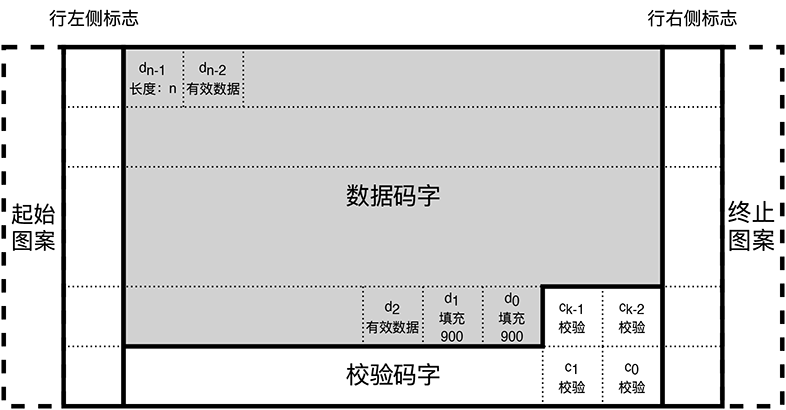
\includegraphics[width=0.95\textwidth]{image/24/3-p-3.png}
\end{figure}

\begin{itemize}
    \item 一个长度码字,表示全部数据码字的个数 $n$,包括该长度码字、有效数据码字、填充码字;
    \item 若干有效数据码字,是此前计算的码字序列;
    \item 零个或多个由重复的 900 组成的填充码字,使得包括校验码字在内的码字总数恰能被有效数据区的行宽度整除。
\end{itemize}

设全部数据码字依次为 $d_{n-1},d_{n-2},\cdots,d_0$
;校验码字依次为 $c_{k-1},c_{k-2},\cdots,c_0$
。那么校验码字按照如下方式计算:

取 $k$ 次多项式 $g(x)=(x-3)(x-3^2)\cdots(x-3^k)$
, $(n-1)$ 次多项式 $d(x)=d_{n-1}x^{n-1}+d_{n-2}x^{n-2}+\cdots+d_1x+d_0$
,找到多项式 $q(x)$ 和不超过 $k-1$ 次的多项式 $r(x)$,使得

\begin{equation*}
    x^kd(x)\equiv q(x)g(x)-r(x)
\end{equation*}

那么多项式 $r(x)$ 中 $x$ 的 $i$ 次项系数对 929 取模后(取正值)的数字即为校验码字 $c_i$
。

例如,如果要将 HE1lo 编码为 PDF417 条码,且有效数据区的行宽是 4 码字(即 68 码元),校验级别为 0。此时校验码字有两个。根据此前的编码结果,有效数据码字有 4 个。再加上一个长度码字,共有 7 个码字。因此需要补充一个填充码字,使包括校验码字在内的总码字数能够被 4 整除。这样,用于计算校验码字的数据码字有 6 个,分别是:

\begin{lstlisting}
    6, 214, 841, 821, 449, 900
\end{lstlisting}

因此有 $g(x)=x^2-12x+27$
,$d(x)=6x^5+214x^4+841x^3+821x^2+449x+900$
,不难得到 $r(x)=-32902164x+98246277$,因此相应可以计算出 $c_1=299\equiv -32902164\mod 929$
,$c_0=811\equiv 98246277\mod 929$
。这样,全部码字序列即为:

\begin{lstlisting}
    6, 214, 841, 821, 449, 900, 229, 811
\end{lstlisting}

在本题中,你需要帮助小 C 完成的任务是,给定被编码的数据,计算出需要填入有效数据区的码字序列。被处理的数据中只含有大写字母、小写字母和数字。

\subsection*{输入格式}

从标准输入读入数据。

输入的第一行包含两个用空格分隔的整数 $w$、$s$,分别表示有效数据区每行能容纳的码字数和校验级别。
保证 $0<w<929$,$-1\le s\le 8$。特别地,当 $s=-1$ 时,表示不需要计算校验码字。

输入的第二行是一个非空字符串,仅包含大小写字母和数字,长度保证编码后全部数据码字的个数少于 929。

\subsection*{输出格式}

输出到标准输出。

输出若干行,每行一个数字,表示编码后的全部码字序列。

\subsection*{样例}

输入\#1:

\begin{lstlisting}
5 -1
HELLO
\end{lstlisting}

输出\#1:

\begin{lstlisting}
5
214
341
449
900
\end{lstlisting}

解释\#1:

要求编码数据是 HELLO,首先查表将其对应成数字。
注意,由于编码器在开始时就处于大写字母模式,因此不需要额外的模式切换。
因此对应成的数字为:7, 4, 11, 11, 14。
由于只有奇数个数字,因此补充 29,形成序列 7, 4, 11, 11, 14, 29。
然后两两成组计算码字:$7\times 30+4=214$,以此类推,得到 214, 341, 449。
本输入不要求产生校验码,且有效数据区的宽度是 5 码字。
目前有效数据的码字是 3 个,加上开头要添加的长度码字,共有 4 个码字。
因此,需要补充一个填充码字,使得总码字数达到 5 个,充满一行。
注意,长度码字中的长度数据包括所有数据码字,因此长度码字是 5 而不是 4。
最终可以得到码字序列 5, 214, 341, 449, 900。

输入\#2:

\begin{lstlisting}
4 0
HE1lo
\end{lstlisting}

输出\#2:

\begin{lstlisting}
6
214
841
821
449
900
229
811
\end{lstlisting}

解释\#2:

本组数据即为此前用于说明编码过程的示例。

\subsection*{子任务}

对于 $20$\% 的数据,有 $s=-1$,且输入字符串中仅含有大写字母或小写字母;

对于 $40$\% 的数据,有 $s=-1$;

对于 $80$\% 的数据,有 $s\le 2$;

对于 $100$\% 的数据,满足全部对于输入的要求。



\section{202112-4 磁盘文件操作}

\subsection*{题目背景}

小C对计算机运行的原理很感兴趣,经常进行一些研究和实验。

有一天,他在尝试删除一个好几GB大小的文件时,惊奇地发现删除操作几乎在一瞬间就完成了!
这让他很是纳闷:如果计算机在每次删除文件时都直接在磁盘上把对应的数据抹掉,不是应该要花挺长时间吗?

于是他找来了小S和小P一起讨论。
小S说,或许计算机是一个很“懒”的体系,在删除时不会真的去抹除数据吧?
而小P则更见多识广一些,他当即找来了一个号称能“恢复磁盘数据”的软件,当场把小C刚刚删除的文件恢复了!

这让小C有了更强的好奇心,于是他们决定设计一个模型来模拟一个磁盘文件的写入、删除及恢复过程。
但是在他们生活的西西艾弗岛上没有合适的条件来运行他们的模型,于是他们联系了带着一台算力超强的电脑来西西艾弗岛旅游的你来帮助他们。

\subsection*{题目描述}

在小C、小S和小P设计的模型中,计算机中有 $n$ 段程序(编号为 $1\sim n$),它们共享一块大小为 $m$ 的磁盘空间(编号为 $1\sim m$ ),磁盘上的每个位置可以写入一个整数。

最初,磁盘上每个位置上的数都是 $0$,并不被任何程序占用。

现在,这 $n$ 段程序同时执行,在某一时刻,某段程序可能对磁盘数据进行读写等操作。

操作共 $k$ 个,按时间先后顺序给出,具体操作如下:

\begin{itemize}
    \item $0\ id\ l\ r\ x$:编号为 $id$ 的程序尝试向磁盘空间中 $[l,r]$ 位置上每个位置都写入一个整数 $x$。
    \begin{itemize}
        \item 操作执行过程中,程序 $id$ 会尝试从最左端 $l$ 开始向右顺次写入数据。
        \item 对于每个位置,若目前不被任何程序占用,则成功写入整数 $x$,并将其视为被程序 $id$ 占用;
        \item 若该位置目前正被程序 $id$ 自己占用,则这次写入的 $x$ 可以覆盖之前写入的结果,此后该位置仍被程序 $id$ 占用;
        \item 直到成功向 $r$ 位置写入数据,或遇到第一个正在被其他程序占用的位置为止,此时该操作立刻中断。
    \end{itemize}
    \item $1\ id\ l\ r$:程序 $id$ 尝试删除磁盘中 $[l,r]$ 位置上的所有数据。
    \begin{itemize}
        \item 这一操作当且仅当 $[l,r]$ 区间内所有位置都正在被程序 $id$ 占用时才能成功执行。
        \item 执行效果为将其中所有位置都解除占用,即恢复到可以被任意程序写入的状态。{\heiti{但为了便于恢复数据,不会立即将全部位置重新覆盖成 $0$}}。
        \item 否则,认为此操作执行失败,不进行任何修改。
    \end{itemize}
    \item $2\ id\ l\ r$:程序 $id$ 尝试恢复磁盘中 $[l,r]$ 位置上的所有数据。
    \begin{itemize}
        \item 这一操作当且仅当 $[l,r]$ 区间内所有位置都未被占用,且{\heiti{上一次被占用是被程序 $id$ 占用}}时才能成功执行。
        \item 执行效果为将其中所有位置恢复为{\heiti{被程序 $id$ 占用}}的状态,同时由于之前删除操作并未改变其存储的值,因此本次操作也不需要改变每个位置上的值。
        \item 否则,认为此操作执行失败,不进行任何修改。
    \end{itemize}
    \item $3\ p$:尝试读取磁盘中 $p$ 位置的数据,返回结果为两个整数。
    \begin{itemize}
        \item 如果该位置当前正被程序 $id$ 占用且存储的值为 $p$,返回结果为 $id\ p$。
        \item 如果该位置当前没有被任何程序占用,返回 $0\ 0$。
    \end{itemize}
\end{itemize}

你需要实现一个程序,帮助小C、小S和小P来模拟实现上述过程,并对于每个操作输出操作结果。

\subsection*{输入格式}

从标准输入读入数据。

第一行:$3$ 个正整数 $n,m,k$。

接下来 $k$ 行,每行若干个整数描述一个操作,格式如上所述。

\subsection*{输出格式}

输出到标准输出。

输出共 $k$ 行,对于每个操作输出一行。

对于每个写入操作,输出一个整数表示此次操作写入成功的最右位置;特别地如果该操作一个位置也没有写入成功,输出 $-1$。

对于每个删除、恢复操作,若该操作成功,输出一个字符串 OK ,否则输出一个字符串 FAIL 。

对于每个读取操作,输出两个整数表示此次查询的结果。

\subsection*{样例}

输入\#1:

\begin{lstlisting}
3 15 12
0 1 1 5 -1
0 2 10 13 2
0 1 4 14 6
1 1 2 8
3 1
3 3
3 14
2 1 3 5
0 3 7 8 -4
2 1 6 8
1 3 6 7
0 2 5 7 3
\end{lstlisting}

输出\#1:

\begin{lstlisting}
5
13
9
OK
1 -1
0 0
0 0
OK
8
FAIL
FAIL
-1
\end{lstlisting}

\subsection*{子任务}

对于 $25$\% 的数据,$n,k\le 2000,m\le 10000$;

对于另外 $15$\% 的数据,没有删除、恢复操作;

对于另外 $20$\% 的数据,没有恢复操作;

对于另外 $15$\% 的数据,$n=1$。

对于 $100$\% 的数据,$1\le n,k\le 2\times 10^5,1\le m\le 10^9,1\le id\le n,1\le l\le r\le m,1\le p\le m,|x|\le 10^9$。



\section{202112-5 极差路径}

\subsection*{题目背景}

众所周知,西西艾弗岛是一个旅游胜地,但是由于兴建机场,西西艾弗岛最近的财务状况有点紧张。

\subsection*{题目描述}

为了从游客手中获取更多的经济利润,岛上仅有的三个小学生小 C、小 S 和小 P 建立了 $n$ 个景点,编号依次从 $1$ 到 $n$。编号为 $i$ 的景点是第 $i$ 个被修建的。
由于越到后期经费越是不足,所以编号更大的景点通常更令人不满意——方便起见,假定编号为 $i$ 的景点的令人不满意程度是 $i$。

有些景点之间修有双向可通行的道路,但是出于减少经费的考虑,他们只修了能使得所有景点连通的最少数量的道路,从而这些景点和其间的道路形成一棵树的结构。

对于每个游客而言,由于只修了 $n-1$ 条道路,所以他只能沿着树上的边参观,并且由于他不可能重复参观一个景点,所以他的游览路径一定是树上的一条简单路径。

现在西西艾弗岛希望制定一些推荐游览路径,但并非所有树上的路径都是合意的,因为这条路径上的景点令人不满意程度的极差可能过大,使游客产生这些景点质量不稳定的错觉。由于最开始的景点和最后的景点令人印象比较深刻,所以游客通常会把游览路径上的景点和这两个景点作比较。因此,最令人不满意的景点不能比这两个景点差太多,最优秀的景点也不能比这两个景点优秀太多。

具体来说,一条从 $x$ 到 $y$ 的游览路径(记作 $(x,y)$)是推荐的,当且仅当下式成立:

\begin{equation*}
    \min\lbrace x,y-k_1\rbrace \le \min\lbrace{P(x,y)}\rbrace \le \max\lbrace{P(x,y)}\rbrace \le \max\lbrace{x,y+k_2}\rbrace
\end{equation*}

其中 $P(x,y)$ 表示一条从 $x$ 出发到达 $y$ 的简单路径上的点的令人不满意程度的数值的集合(包括 $x$ 和 $y$,也就是 $x$ 到 $y$ 的简单路径上的点的编号的集合),$\min S$ 和 $\max S$ 分别表示集合 $S$ 中的最小和最大值,$k_1,k_2$ 是西西艾弗岛经过数次尝试后选取的两个给定的参数,保证 $k_1,k_2>0$。

特别的,容易验证 $x=y$ 时 $(x,y)$ 总是推荐的。

现在西西艾弗岛想知道,一共有多少树上的简单路径作为游览路径是被推荐的?这里我们认为 $(x,y)$ 和 $(y,x)$ 是同一条路径。

\subsection*{输入格式}

从标准输入读入数据。

第一行输入三个非负整数 $n,k_1,k_2$。

接下来 $n-1$ 行,每行两个正整数 $x,y$ 表示树上的一条边。

\subsection*{输出格式}

输出到标准输出。

输出一行一个非负整数表示答案。

\subsection*{样例}

输入\#1:

\begin{lstlisting}
5 0 1
5 4
4 2
4 1
2 3
\end{lstlisting}

输出\#1:

\begin{lstlisting}
12
\end{lstlisting}

解释\#1:

容易验证 $(1,1),(1,4),(1,5),(1,3),(2,2),(2,4),(2,5),(2,3),(3,3),(4,4),(4,5),(5,5)$ 都是推荐的游览路径,因此答案是 $12$。

\subsection*{子任务}

\begin{table}[H]
\centering
\begin{tabular}{cccccc}
    \toprule
    测试点 & $n\le$ & $k_1$ & $k_2$ & 树的形态 & 堆性质 \\
    \midrule
    $1$ & $5000$ & $\le n$ & $\le n$ & $A_3$ & 无 \\
    $2$ & $5000$ & $\le n$ & $\le n$ & $A_3$ & 无 \\
    $3$ & $5000$ & $\le n$ & $\le n$ & $A_3$ & 无 \\
    $4$ & $5\times 10^5$ & $=0$ & $=0$ & $A_1$ & 有 \\
    $5$ & $5\times 10^5$ & $=0$ & $=0$ & $A_1$ & 无 \\
    $6$ & $5\times 10^5$ & $\le n$ & $=0$ & $A_1$ & 有 \\
    $7$ & $5\times 10^5$ & $\le n$ & $=0$ & $A_1$ & 无 \\
    $8$ & $5\times 10^5$ & $\le n$ & $\le n$ & $A_1$ & 有 \\
    $9$ & $5\times 10^5$ & $\le n$ & $\le n$ & $A_1$ & 无 \\
    $10$ & $5\times 10^5$ & $=0$ & $=0$ & $A_2$ & 无 \\
    $11$ & $5\times 10^5$ & $\le n$ & $=0$ & $A_2$ & 无 \\
    $12$ & $5\times 10^5$ & $\le n$ & $\le n$ & $A_2$ & 无 \\
    $13$ & $5\times 10^5$ & $=0$ & $=0$ & $A_3$ & 有 \\
    $14$ & $5\times 10^5$ & $=0$ & $=0$ & $A_3$ & 无 \\
    $15$ & $5\times 10^5$ & $=0$ & $=0$ & $A_3$ & 无 \\
    $16$ & $5\times 10^5$ & $=0$ & $=0$ & $A_3$ & 无 \\
    $17$ & $5\times 10^5$ & $\le n$ & $=0$ & $A_3$ & 有 \\
    $18$ & $5\times 10^5$ & $\le n$ & $=0$ & $A_3$ & 无 \\
    $19$ & $5\times 10^5$ & $\le n$ & $=0$ & $A_3$ & 无 \\
    $20$ & $5\times 10^5$ & $\le n$ & $=0$ & $A_3$ & 无 \\
    $21$ & $5\times 10^5$ & $\le n$ & $\le n$ & $A_3$ & 有 \\
    $22$ & $5\times 10^5$ & $\le n$ & $\le n$ & $A_3$ & 有 \\
    $23$ & $5\times 10^5$ & $\le n$ & $\le n$ & $A_3$ & 无 \\
    $24$ & $5\times 10^5$ & $\le n$ & $\le n$ & $A_3$ & 无 \\
    $25$ & $5\times 10^5$ & $\le n$ & $\le n$ & $A_3$ & 无 \\
    \bottomrule
\end{tabular}
\end{table}

对于 $100$\% 的数据,$1\le n\le 5\times 10^5,0\le k_1,k_2\le n$,保证输入的 $n-1$ 条边一定构成一棵树。

树的形态:

\begin{itemize}
    \item $A_1$:树是一条链;
    \item $A_2$:存在一个度数为 $n-1$ 的点;
    \item $A_3$:树的形态无特殊性质。
\end{itemize}

堆性质:若取编号为 $1$ 的点为根,则除 $1$ 号点外,每个点的编号都比其父节点的编号大。

\subsection*{提示}

请注意答案可能的取值范围。



\end{document}
